\documentclass[twoside,english]{uiofysmaster}

%\usepackage[utf8]{inputenc} % Riktig tegnsett
\usepackage{babel} 
\usepackage{url}
\usepackage{units}
\usepackage{lipsum}
\usepackage{graphicx}  
\usepackage{subcaption} 
\usepackage{color}
\usepackage{amsmath}  
\usepackage{hyperref}
\usepackage{braket} 
\usepackage{multicol}
%\usepackage{listings}  
\usepackage{amsfonts}
%\usepackage{siunitx}
\usepackage{float}
\usepackage{HASstyle}
% Custom commands
\newcommand\lr[1]{\left(#1\right)} 

\definecolor{LightBlue}{rgb}{0.8, 0.8, 0.95}

\definecolor{editColor}{rgb}{0.5, 0.0, 0.0}


\author{Filip Henrik Larsen}
\title{Title of the master thesis}
\date{May 2017}

\begin{document}

\maketitle

\begin{abstract}
This is an abstract text.
\end{abstract}

\begin{dedication}
  To someone
  \\\vspace{12pt}
  This is a dedication to my cat.
\end{dedication}

\begin{acknowledgements}
  Flora Joelle Larsen\\*
  Anders Hafreager
\end{acknowledgements}

\tableofcontents

\chapter{Introduction}

Why is the subject of this thesis of any interest?\\
What is our take on the problem?\\
What do we hope to accomplish?\\
How will this be of any contribution to anything?\\
How is the thesis laid out?



\chapter{LAMMPS}

LAMMPS stands for \textit{Large-scale Atomic/Molecular Massively Parallel Simulator}. It is a classical molecular dynamics simulation code designed to run efficiently on parallel computers. It's development began in the mid 1990s at Sandia National Laboratories, with funding from the U.S. Department of Energy. It was a cooperative project between two DOE labs and three private companies. The development is still ongoing and contributions are revised thoroughly. 

Today LAMMPS is an open-source code with extensive and user friendly documentation. This is one of the main reasons that we have chosen to use LAMMPS as opposed to other molecular dynamics software. 

\section{Installation}
Installing LAMMPS is a fairly simple procedure if only the basic settings are needed.

\subsection{Linux}
Users with a Unix based OS may download the lammps distribution as a tarball from LAMMPS' download page\footnote{\href{http://lammps.sandia.gov/download.html}{http://lammps.sandia.gov/download.html}} and then unpack it from the command line.
\begin{lstlisting}
gunzip filename.tar.gz
tar xvf filename.tar
\end{lstlisting}
The user may then change directory into \texttt{/path/to/lammps/src/}, and execute the following commands in order to list available packages. 
\begin{lstlisting}
make package-status
\end{lstlisting}
Installing specific packages is accomplished as shown below.
\begin{lstlisting}
make yes-molecule yes-manybody yes-python yes-rigid 
\end{lstlisting}
The above example installs the packages \textit{molecule, manybody, python and rigid}.
Next, the user can build LAMMPS using either of the lines below. Assuming the user has MPI installed line 2 makes the resulting executable compatible with parallelization in MPI.
\begin{lstlisting}
make serial
make mpi
\end{lstlisting}
At this point there should be an executable in the \texttt{/path/to/lammps/src/} directory named \texttt{lmp\_serial} or \texttt{lmp\_mpi}, depending on the previous choice. These are now ready to run.
To use it one has to point to this file from the command line at every run. It may be practical to set up a symlink as follows shown below.

\begin{lstlisting}
sudo ln -s /path/to/lammps/src/lmp_mpi /usr/local/bin/lmp_mpi
\end{lstlisting}
The executable is now available as \texttt{lmp\_serial} or \texttt{lmp\_mpi} from anywhere.

\subsection{Mac OS X with Homebrew}
Mac users can follow the procedure described above, however they may also install even easier using \textit{Homebrew}\footnote{\href{http://brew.sh/}{http://brew.sh/}}. 
\begin{lstlisting}
brew tap homebrew/science
brew install lammps              # serial version
brew install lammps --with-mpi   # mpi support 
\end{lstlisting}
Where the user obviously should choose either line 2 or line 3, depending on if the user wants MPI comparability.
This will install an executable named "lammps", a python module named "lammps", and resources with standard packages. 
This is basically it. LAMMPS is now ready to run, however, not all packages are installed.

The location of the resources and available packages can be found using the following command.
\begin{lstlisting}
brew info lammps 
\end{lstlisting}
Specific packages are available as options, and may be installed with the following command.

\begin{lstlisting}
brew install lammps --enable-manybody 
\end{lstlisting}
In the example shown we installed the package manybody.


\subsection{Windows}



\section{Running LAMMPS}




\section{Creating a custom compute}
A \textit{compute} is a LAMMPS command that defines a computation that will be performed on a group of atoms. The \textit{computes} produce instantaneous values, using information about the atoms on the current time step. 

In LAMMPS there are more than 100 computes already, and chances are they have what you're looking for. If not, one might treat the data from other computes in some way to get the desired information. However, if there are no compute command that does the desired task, it is possible to create an own custom class.  

In order to compute the normal forces acting on the sphere, we have written a custom compute class. The purpose of the class was to save the forces acting on atoms in one group from atoms of another group. In this section we will try do give brief instructions on how this was done.

[MAYBE A FIGURE HERE]

\subsection{Find a similar compute}
Obviously, before writing any code we should know what we want the compute to calculate and how this should be done. 
Before starting off with a blank sheet in the editor, one should definitely search for similar computes in LAMMPS. This can potentially save hours of hard work!

For instance there is a compute named \textit{group/group}\footnote{\href{http://lammps.sandia.gov/doc/compute_group_group.html}{http://lammps.sandia.gov/doc/compute\_group\_group.html}} which computes the total energy and force interaction between two groups of atoms. This is almost what we want, but we also need to know how many atoms contribute to this total force, and it should also work with the Vashishta potential. {\color{red} ++}

Thus there are minor modifications needed, and we chose to make our compute a subclass of this one.


\subsection{Creating the class}
All computes in LAMMPS are subclasses of the class named  \textit{compute}. From this superclass they inherit a bunch of variables, functions and flags, which the user may decide to set. Functions are of course declared in the \texttt{.h}-file, while variables and flags are set in the constructor. The source code of the \textit{group/group} compute is shown in Appendix \ref{groupgrouph}. The only modification of this file is the change from private to protected property of some variables.
We start out by creating a header file, and decide upon a name for our class. We have chosen the name \textit{group/group/atom} since it is basically a per-atom version of \textit{group/group}.

\lstinputlisting[caption={},language=c++, firstline=14, lastline=40]{../../LAMMPS/src/compute_group_group_atom.h}










\chapter{Setting up the system}

We wish to construct a system consisting of {\color{red} two} elements made out of silica: a slab and a sphere cap. In order to do this we need to generate the spacial position coordinates (x,y,z) of every single atom. Considering that we are making a system consisting of about $10^5$ atoms, this is obviously not done manually. We have chosen to use a tool named \textit{Moltemplate}\footnote{\href{http://www.moltemplate.org/index.html}{http://www.moltemplate.org/index.html}}, which is included in the LAMMPS distribution.

The main idea is to manually enter the coordinates of only the atoms in a unit cell of the material one wish to generate, and then simply copy this unit cell wherever desired. The software will shift the coordinates of the copied unit cell by the displacement from the original image. In addition it will generate files containing data such as which atoms they share bonds with, if any, and angles between such bonds. 

\section{Silica}
Silica is a chemical compound also known as Silicon dioxide, having the chemical formula SiO$_2$. It has several polymorph structures, the most common being quartz, which is one of the most abundant minerals in the Earth's crust. Other polymorphs include cristobalite, tridymite, coesite and more.    

For our purpose it is insignificant which one we choose. Once the material is melted, it is indifferent which configuration we started from, as long as the density is correct.
In this project we will build the constituents of the system from a type of cristobalite named $\beta$-cristobalite. This is mainly because it has a simple structure and a cubical unit cell.


\subsection{Unit cell of $\beta$-cristobalite}
In order to construct the unit cell of a material, one should look up the coordinates of the atoms in a crystallography database. We have used the unit cell of $\beta$-cristobalite found at \textit{Crystallography Open Database}\footnote{\href{http://www.crystallography.net/cod/1010944.html}{http://www.crystallography.net/cod/1010944.html}}. At this site one can download a \texttt{.cif}-file consisting of the spatial positions of each atom, the length of the unit cell edges and angles between faces of the cell. In the case of $\beta$-cristobalite the unit cell is cubical with edges of length 7.12Å. It contain 8 silicon atoms and 16 oxygen atoms. The density of the unit cell can easily be computed and is 2.2114 g/cm$^3$.

\begin{figure}
	\centering
	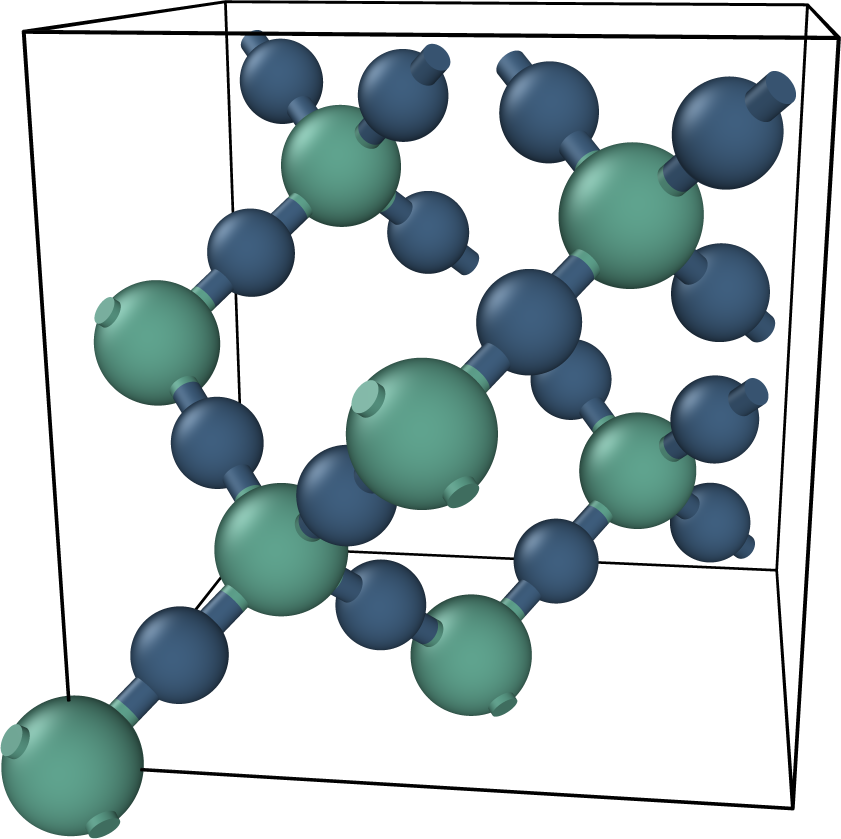
\includegraphics[width=0.7\linewidth]{figures/unitcell/unitcell.png}
	\caption{Unit cell of b-cristobalite. Tan and blue spheres represent silicon and oxygen atoms respectively.}
	\label{fig:unitcellbcristobalite}
\end{figure}



\section{Building a crystal}
The coordinates gotten from the \texttt{.cif}-file can now be implemented into \textit{moltemplate} together with whatever bond and angle data required by the potential. In our simulations we will use the Vashishta potential, which does not require these. 

Moltemplate has its own structure and syntax. The first step to build up a larger material is, as mentioned, to create the unit cell. Data concerning the unit cell are placed in a \texttt{.lt}-file, which is readable by Moltemplate. Such a file is shown in Listing \ref{lst:beta-cristobalite.lt}. 

For a more profound understanding of the structure and syntax of these files, the reader is advised to read the moltemplate manual  

\begin{center}
\begin{minipage}{\linewidth}
	\lstinputlisting[caption={Typical moltemplate file containing unit cell data. The columns of the "Data Atoms" section hold, from left to right, information of atom ID, atom type, x-, y- and z-position. The "Data Masses" section stores the weight of silicon and oxygen atoms in atomic mass units.}, label=lst:beta-cristobalite.lt,
	language=LammpsData]{../SiO2/large/beta-cristobalite.lt}
\end{minipage}
\end{center}

We use the unit cell as building blocks, placing them concurrently until we have a crystal of the desired size. For our purpose, we generate a large cube of $15\times15\times15$ unit cells. This is done as follows.



\begin{figure}
	\centering
	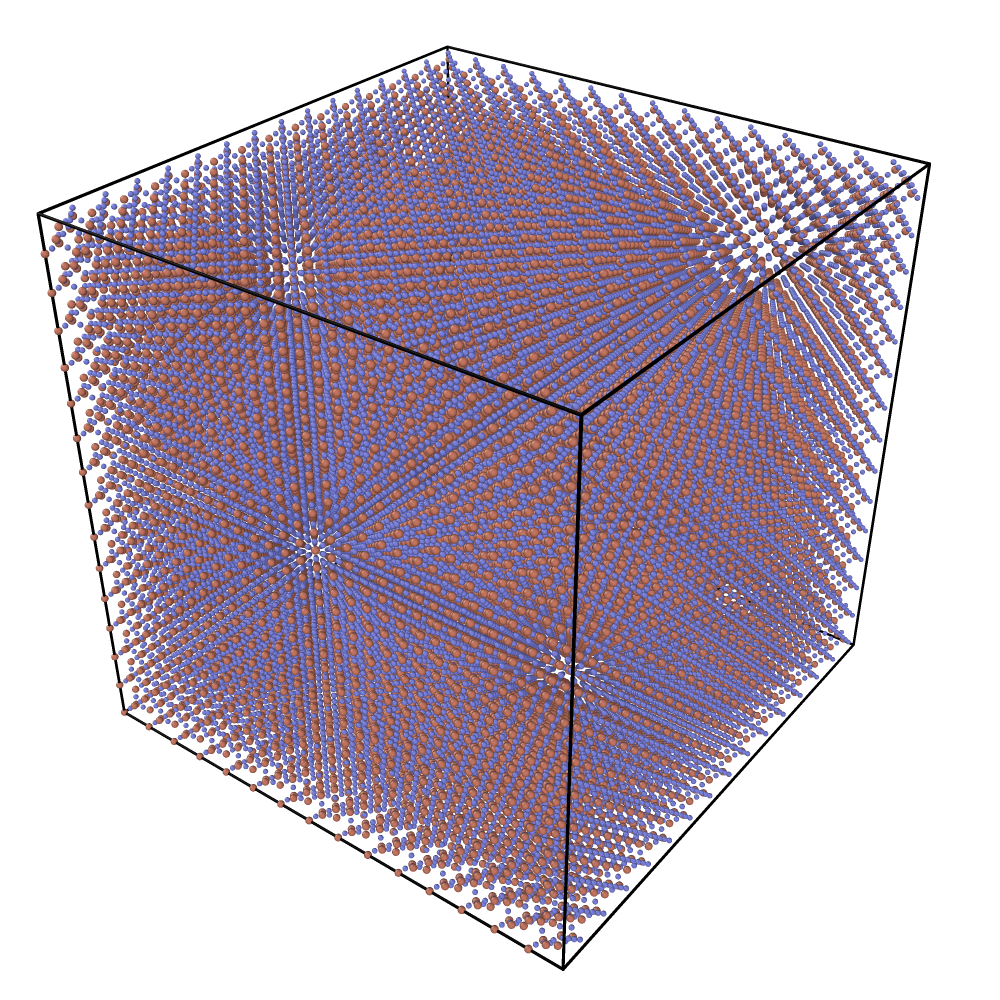
\includegraphics[width=0.7\linewidth]{figures/CreatingSystem/hugeCube}
	\caption{System built from $15\times15\times15$ unit cells of b-cristobalite.}
	\label{fig:hugeCube}
\end{figure}

\section{Shaping the silica}

\begin{figure}
	\centering
	
\includegraphics[width=0.7\linewidth]{figures/CreatingSystem/drawing.pdf}
	\caption{Illustrative drawing of what how the system should look. Red parallel stripes symbolize areas of silica. Red crossing stripes indicate areas of frozen silica. The boundaries are periodic in all dimensions, causing both the slab and the sphere to be connected to the frozen silica through the z-boundaries.}
	\label{fig:drawing}
\end{figure}

The huge cube of silica can be carved however we like by defining regions from which we delete the containing atoms. In LAMMPS this is done by using the \texttt{region}, \texttt{union}, \texttt{intersect} and \texttt{delete atoms} commands. Our implementation is stated in Listing \ref{lst:sculpting}, which is very simple due to the way we are going to treat the boundary conditions. 

\lstinputlisting[caption={Defining regions to keep or delete from a system of dimensions $106.8\times106.8\times106.8$ Å.}, label={lst:sculpting}]{../SiO2/small/system.prepare.latex}



\chapter{This must be sorted in designated chapters}

\section{Radial distribution of normal force}
In order to find a radial distribution of the normal force, $F_N$, we partition the system into a grid in  the xy-plane. We then use the command 

\begin{lstlisting}[language=LammpsInput]
	compute chunkID all chunk/atom bin/2d x 0 7.12 y 0 7.12
	compute stressID all stress/atom NULL
	fix fixChunkID all ave/chunk 1 1 10 chunkID c_stressID[3] file forcesInChunks.txt
\end{lstlisting} 
to compute the stress of every chunk in the z-direction, $\sigma_{zz}$ (sum of every individual atom stress in the chunk). 

Line 1 establishes the grid, with bin width $7.12$Å.

Line 2 creates a compute of the stress

Line 3 stores the sum of individual stresses in each chunk to the file \texttt{forcesInChunks.txt}. 
This is done every 10 time steps in order to reduce correlation effects. 

The data in stored from each time step can easily be averaged to produce a result as shown in figure X.

We can then find the radial distribution simply by binning this matrix in radial bins, and average the normal forces of the chunks within the bins.


% ---------------------------------------------------------------------------- %

\appendix
\chapter{Source code}

\newpage
\section{compute\_group\_group.h}
\label{groupgrouph}
\lstinputlisting[language=c++, firstline=14, lastline=53]{../../LAMMPS/src/compute_group_group.h}

\newpage
\section{compute\_group\_group\_atom.h}
\lstinputlisting[language=c++, firstline=14, lastline=40]{../../LAMMPS/src/compute_group_group_atom.h}


\newpage
\section{compute\_group\_group\_atom.cpp}
\lstinputlisting[language=c++, firstline=19]{../../LAMMPS/src/compute_group_group_atom.cpp}


\bibliography{resources/Library.bib}


%Referances






\end{document}
```

Centering the front page
------------------------
By default, the maketitle command will generate the front page, but it will not be properly centered, but offset like any other page. To get around this, the best solution is to create a separate document, name it front-page.tex and add the following to it:

front-page.tex:
```latex
\documentclass[twoside,english]{uiofysmaster}
\geometry{a4paper,includeall,bindingoffset=0cm,margin=3cm,
            marginparsep=0cm,marginparwidth=0cm,top=2cm}

\author{Filip Henrik Larsen}
\title{\uppercase{The history of master thesises and other random gibberish}}
\date{June 2012}

\begin{document}

\begin{titlepage}
\maketitle
\end{titlepage}

\end{document}
